\subsection{Efficienza locale}
\label{localis}
Utilizzando gli stessi dati della \autoref{attenu}, abbiamo studiato le variazioni di efficienza in vari punti del PM1. In \autoref{capolavoro} è presente un grafico 3D che mostra i conteggi ottenuti in ogni casella in cui è stato posizionato il miniscint. Si può apprezzare una diminuzione dei conteggi tra le varie colonne per i motivi discussi in \autoref{attenu} ma è anche evidente come all'interno di una stessa colonna ci siano delle variazioni significative tra una riga e l'altra.
\marginpar{Non so cosa scrivere. Se lo sapete scrivetelo. Io intanto lavoro su altro.}
\begin{figure}[h]
\flushleft
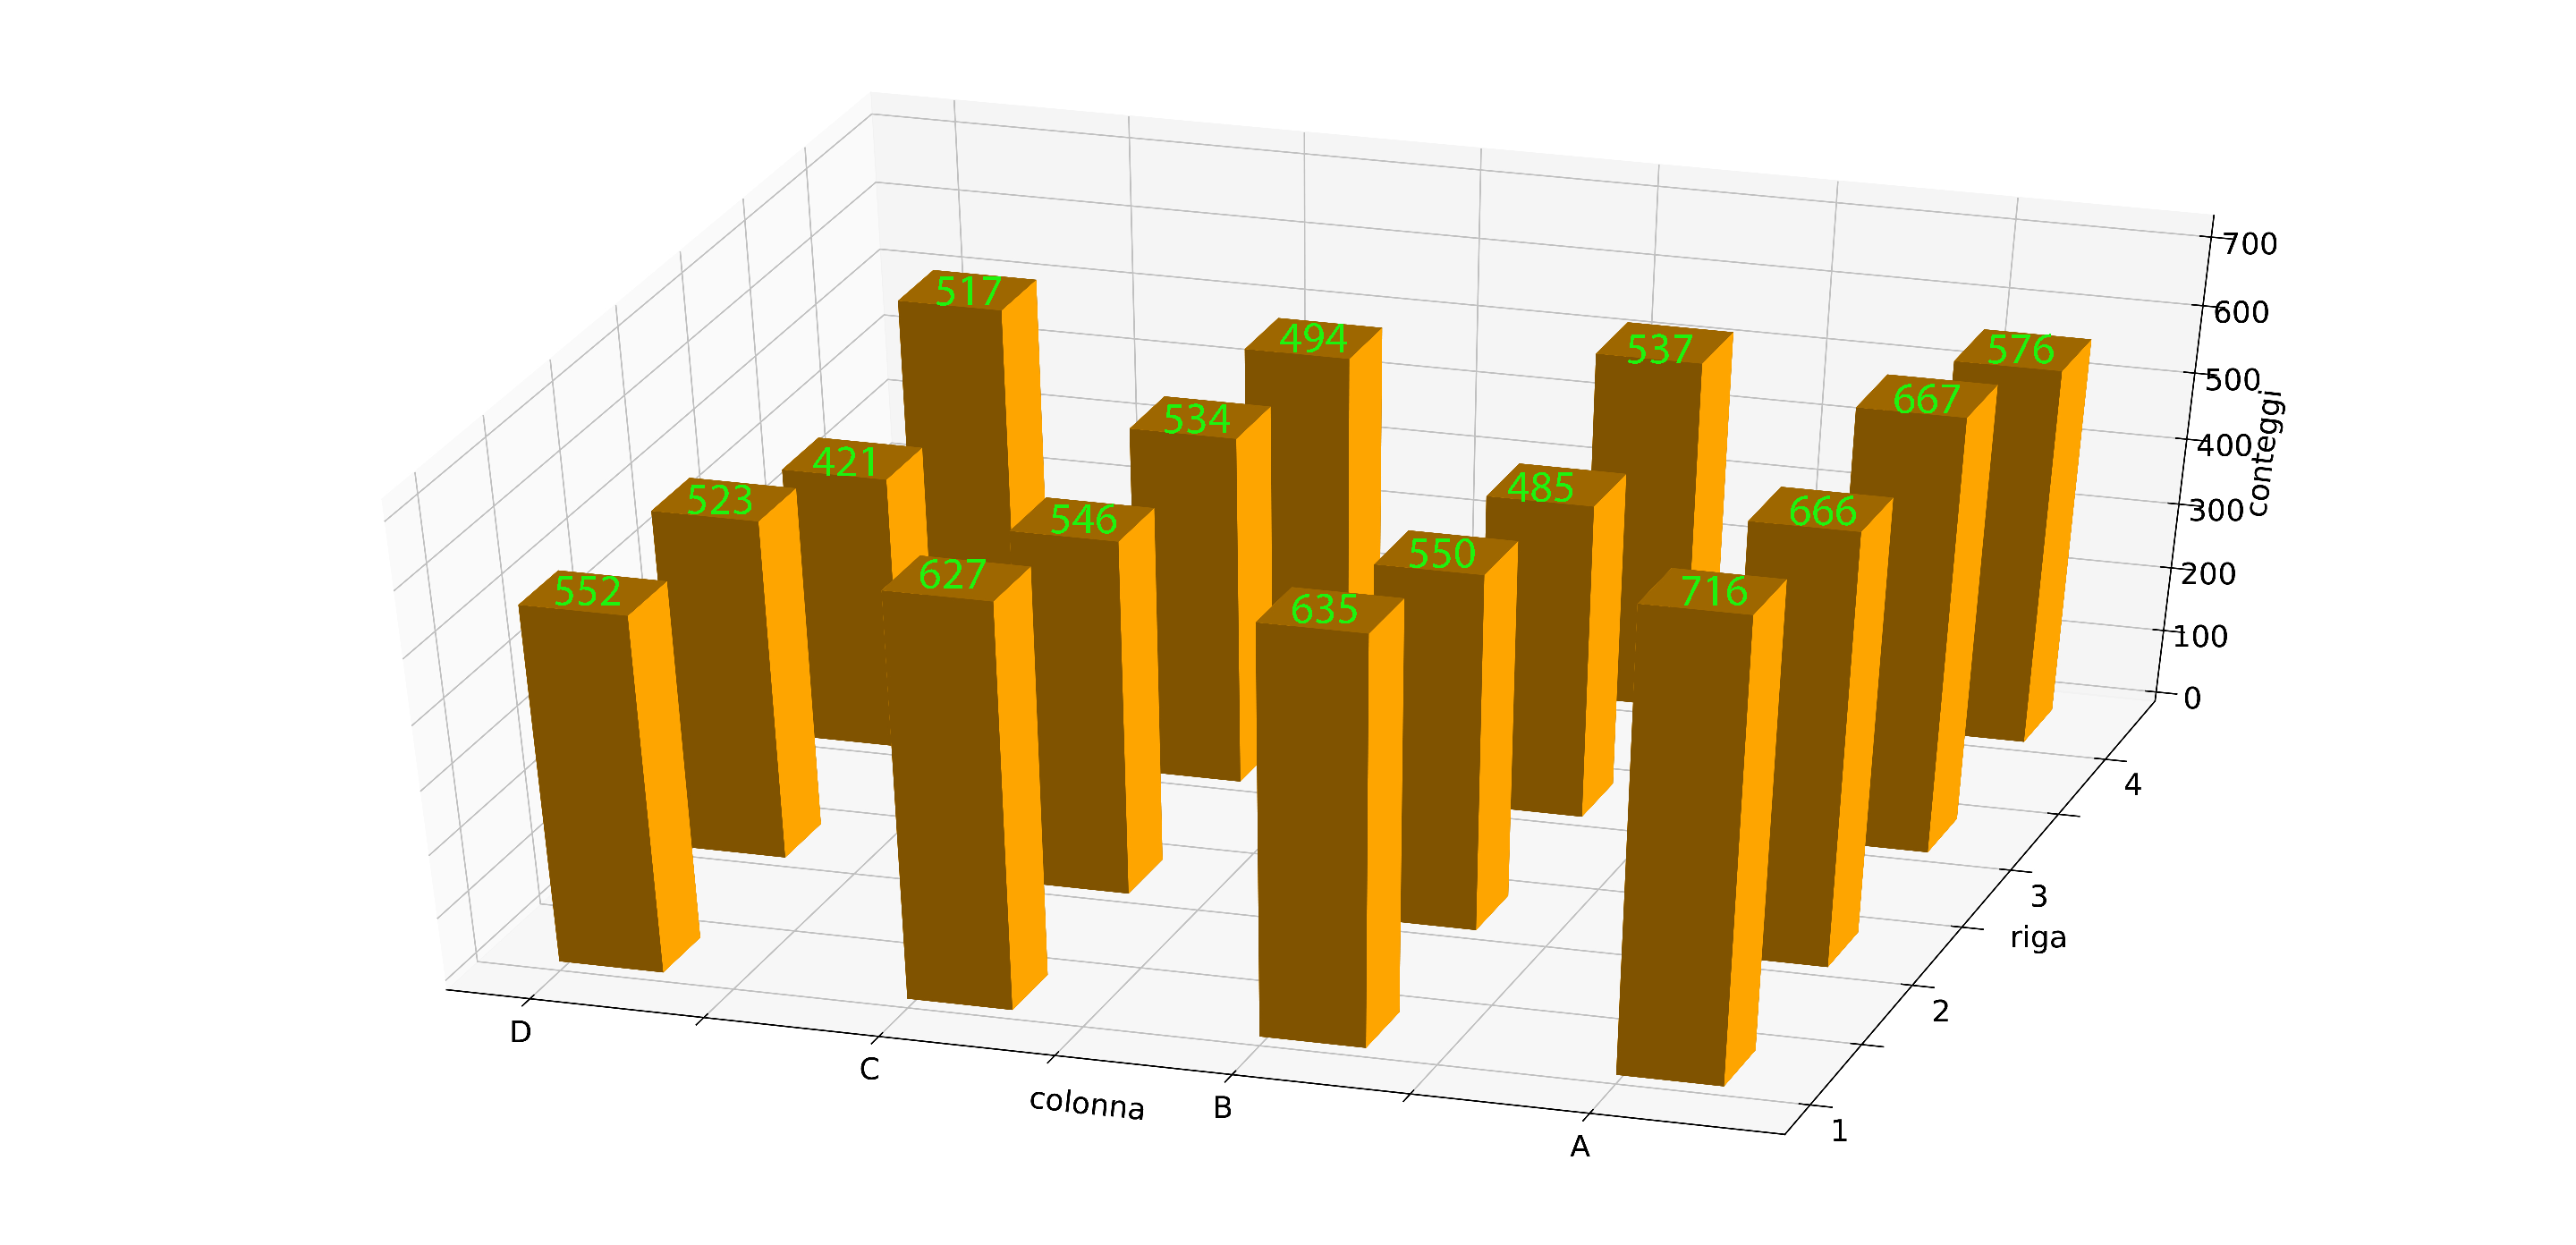
\includegraphics[width=17 cm]{3d_rit}
\caption{Conteggi PM1 nelle rispettive caselle. L'errore su ogni conteggio è la radice quadrata dello stesso. La disposizione delle caselle è la stessa che in quel disegno che Jack farà perché è bravo a disegnare anche al computer.}
\label{capolavoro}
\end{figure}

Per meglio comprendere la situazione, dividiamo tutti i conteggi per quello più alto, in modo da vedere le variazioni percentuali tra una casella e l'altra del PM1. Il grafico a barre di \autoref{secondo_capolavoro} mostra il risultato ottenuto e la \autoref{auto} riporta i valori dei singoli punti con il loro errore.

\begin{table}[h]
\centering
\begin{tabular}{|c|c|c|c|c|}
\hline
colonna & D & C & B & A \\
 \hline
riga  & & & &  \\
1 &  $ 0.77 \pm 0.04 $ & $ 0.88 \pm 0.05 $ & $ 0.89 \pm 0.05 $ & $ 1 \pm 0 $ \\ 
2 &  $ 0.73 \pm 0.04 $ & $ 0.76 \pm 0.04 $ & $ 0.77 \pm 0.04 $ & $ 0.93 \pm 0.05 $ \\ 
3 &  $ 0.59 \pm 0.04 $ & $ 0.75 \pm 0.04 $ & $ 0.68 \pm 0.04 $ & $ 0.93 \pm 0.05 $ \\ 
4 &  $ 0.72 \pm 0.04 $ & $ 0.69 \pm 0.04 $ & $ 0.75 \pm 0.04 $ & $ 0.80 \pm 0.05 $ \\
\hline 
\end{tabular}
\caption{conteggi normalizzati nelle varie caselle del PM1.}
\label{auto}
\end{table}

\begin{figure}[h]
\flushleft
\includegraphics[width=17 cm]{3d_norm_rit}
\caption{Conteggi normalizzati PM1 nelle rispettive caselle.}
\label{secondo_capolavoro}
\end{figure}

